\documentclass{ximera}

%\usepackage{todonotes}

\newcommand{\todo}{}

\usepackage{esint} % for \oiint
\ifxake%%https://math.meta.stackexchange.com/questions/9973/how-do-you-render-a-closed-surface-double-integral
\renewcommand{\oiint}{{\large\bigcirc}\kern-1.56em\iint}
\fi


\graphicspath{
  {./}
  {ximeraTutorial/}
  {basicPhilosophy/}
  {functionsOfSeveralVariables/}
  {normalVectors/}
  {lagrangeMultipliers/}
  {vectorFields/}
  {greensTheorem/}
  {shapeOfThingsToCome/}
  {dotProducts/}
  {partialDerivativesAndTheGradientVector/}
  {../productAndQuotientRules/exercises/}
  {../normalVectors/exercisesParametricPlots/}
  {../continuityOfFunctionsOfSeveralVariables/exercises/}
  {../partialDerivativesAndTheGradientVector/exercises/}
  {../directionalDerivativeAndChainRule/exercises/}
  {../commonCoordinates/exercisesCylindricalCoordinates/}
  {../commonCoordinates/exercisesSphericalCoordinates/}
  {../greensTheorem/exercisesCurlAndLineIntegrals/}
  {../greensTheorem/exercisesDivergenceAndLineIntegrals/}
  {../shapeOfThingsToCome/exercisesDivergenceTheorem/}
  {../greensTheorem/}
  {../shapeOfThingsToCome/}
  {../separableDifferentialEquations/exercises/}
  {vectorFields/}
}

\newcommand{\mooculus}{\textsf{\textbf{MOOC}\textnormal{\textsf{ULUS}}}}

\usepackage{tkz-euclide}
\usepackage{tikz}
\usepackage{tikz-cd}
\usetikzlibrary{arrows}
\tikzset{>=stealth,commutative diagrams/.cd,
  arrow style=tikz,diagrams={>=stealth}} %% cool arrow head
\tikzset{shorten <>/.style={ shorten >=#1, shorten <=#1 } } %% allows shorter vectors

\usetikzlibrary{backgrounds} %% for boxes around graphs
\usetikzlibrary{shapes,positioning}  %% Clouds and stars
\usetikzlibrary{matrix} %% for matrix
\usepgfplotslibrary{polar} %% for polar plots
\usepgfplotslibrary{fillbetween} %% to shade area between curves in TikZ
%\usetkzobj{all}
\usepackage[makeroom]{cancel} %% for strike outs
%\usepackage{mathtools} %% for pretty underbrace % Breaks Ximera
%\usepackage{multicol}
\usepackage{pgffor} %% required for integral for loops



%% http://tex.stackexchange.com/questions/66490/drawing-a-tikz-arc-specifying-the-center
%% Draws beach ball
\tikzset{pics/carc/.style args={#1:#2:#3}{code={\draw[pic actions] (#1:#3) arc(#1:#2:#3);}}}



\usepackage{array}
\setlength{\extrarowheight}{+.1cm}
\newdimen\digitwidth
\settowidth\digitwidth{9}
\def\divrule#1#2{
\noalign{\moveright#1\digitwidth
\vbox{\hrule width#2\digitwidth}}}




% \newcommand{\RR}{\mathbb R}
% \newcommand{\R}{\mathbb R}
% \newcommand{\N}{\mathbb N}
% \newcommand{\Z}{\mathbb Z}

\newcommand{\sagemath}{\textsf{SageMath}}


%\renewcommand{\d}{\,d\!}
%\renewcommand{\d}{\mathop{}\!d}
%\newcommand{\dd}[2][]{\frac{\d #1}{\d #2}}
%\newcommand{\pp}[2][]{\frac{\partial #1}{\partial #2}}
% \renewcommand{\l}{\ell}
%\newcommand{\ddx}{\frac{d}{\d x}}

% \newcommand{\zeroOverZero}{\ensuremath{\boldsymbol{\tfrac{0}{0}}}}
%\newcommand{\inftyOverInfty}{\ensuremath{\boldsymbol{\tfrac{\infty}{\infty}}}}
%\newcommand{\zeroOverInfty}{\ensuremath{\boldsymbol{\tfrac{0}{\infty}}}}
%\newcommand{\zeroTimesInfty}{\ensuremath{\small\boldsymbol{0\cdot \infty}}}
%\newcommand{\inftyMinusInfty}{\ensuremath{\small\boldsymbol{\infty - \infty}}}
%\newcommand{\oneToInfty}{\ensuremath{\boldsymbol{1^\infty}}}
%\newcommand{\zeroToZero}{\ensuremath{\boldsymbol{0^0}}}
%\newcommand{\inftyToZero}{\ensuremath{\boldsymbol{\infty^0}}}



% \newcommand{\numOverZero}{\ensuremath{\boldsymbol{\tfrac{\#}{0}}}}
% \newcommand{\dfn}{\textbf}
% \newcommand{\unit}{\,\mathrm}
% \newcommand{\unit}{\mathop{}\!\mathrm}
% \newcommand{\eval}[1]{\bigg[ #1 \bigg]}
% \newcommand{\seq}[1]{\left( #1 \right)}
% \renewcommand{\epsilon}{\varepsilon}
% \renewcommand{\phi}{\varphi}


% \renewcommand{\iff}{\Leftrightarrow}

% \DeclareMathOperator{\arccot}{arccot}
% \DeclareMathOperator{\arcsec}{arcsec}
% \DeclareMathOperator{\arccsc}{arccsc}
% \DeclareMathOperator{\si}{Si}
% \DeclareMathOperator{\scal}{scal}
% \DeclareMathOperator{\sign}{sign}


%% \newcommand{\tightoverset}[2]{% for arrow vec
%%   \mathop{#2}\limits^{\vbox to -.5ex{\kern-0.75ex\hbox{$#1$}\vss}}}
% \newcommand{\arrowvec}[1]{{\overset{\rightharpoonup}{#1}}}
% \renewcommand{\vec}[1]{\arrowvec{\mathbf{#1}}}
% \renewcommand{\vec}[1]{{\overset{\boldsymbol{\rightharpoonup}}{\mathbf{#1}}}}

% \newcommand{\point}[1]{\left(#1\right)} %this allows \vector{ to be changed to \vector{ with a quick find and replace
% \newcommand{\pt}[1]{\mathbf{#1}} %this allows \vec{ to be changed to \vec{ with a quick find and replace
% \newcommand{\Lim}[2]{\lim_{\point{#1} \to \point{#2}}} %Bart, I changed this to point since I want to use it.  It runs through both of the exercise and exerciseE files in limits section, which is why it was in each document to start with.

% \DeclareMathOperator{\proj}{\mathbf{proj}}
% \newcommand{\veci}{{\boldsymbol{\hat{\imath}}}}
% \newcommand{\vecj}{{\boldsymbol{\hat{\jmath}}}}
% \newcommand{\veck}{{\boldsymbol{\hat{k}}}}
% \newcommand{\vecl}{\vec{\boldsymbol{\l}}}
% \newcommand{\uvec}[1]{\mathbf{\hat{#1}}}
% \newcommand{\utan}{\mathbf{\hat{t}}}
% \newcommand{\unormal}{\mathbf{\hat{n}}}
% \newcommand{\ubinormal}{\mathbf{\hat{b}}}

% \newcommand{\dotp}{\bullet}
% \newcommand{\cross}{\boldsymbol\times}
% \newcommand{\grad}{\boldsymbol\nabla}
% \newcommand{\divergence}{\grad\dotp}
% \newcommand{\curl}{\grad\cross}
%\DeclareMathOperator{\divergence}{divergence}
%\DeclareMathOperator{\curl}[1]{\grad\cross #1}
% \newcommand{\lto}{\mathop{\longrightarrow\,}\limits}

% \renewcommand{\bar}{\overline}

\colorlet{textColor}{black}
\colorlet{background}{white}
\colorlet{penColor}{blue!50!black} % Color of a curve in a plot
\colorlet{penColor2}{red!50!black}% Color of a curve in a plot
\colorlet{penColor3}{red!50!blue} % Color of a curve in a plot
\colorlet{penColor4}{green!50!black} % Color of a curve in a plot
\colorlet{penColor5}{orange!80!black} % Color of a curve in a plot
\colorlet{penColor6}{yellow!70!black} % Color of a curve in a plot
\colorlet{fill1}{penColor!20} % Color of fill in a plot
\colorlet{fill2}{penColor2!20} % Color of fill in a plot
\colorlet{fillp}{fill1} % Color of positive area
\colorlet{filln}{penColor2!20} % Color of negative area
\colorlet{fill3}{penColor3!20} % Fill
\colorlet{fill4}{penColor4!20} % Fill
\colorlet{fill5}{penColor5!20} % Fill
\colorlet{gridColor}{gray!50} % Color of grid in a plot

\newcommand{\surfaceColor}{violet}
\newcommand{\surfaceColorTwo}{redyellow}
\newcommand{\sliceColor}{greenyellow}




\pgfmathdeclarefunction{gauss}{2}{% gives gaussian
  \pgfmathparse{1/(#2*sqrt(2*pi))*exp(-((x-#1)^2)/(2*#2^2))}%
}


%%%%%%%%%%%%%
%% Vectors
%%%%%%%%%%%%%

%% Simple horiz vectors
\renewcommand{\vector}[1]{\left\langle #1\right\rangle}


%% %% Complex Horiz Vectors with angle brackets
%% \makeatletter
%% \renewcommand{\vector}[2][ , ]{\left\langle%
%%   \def\nextitem{\def\nextitem{#1}}%
%%   \@for \el:=#2\do{\nextitem\el}\right\rangle%
%% }
%% \makeatother

%% %% Vertical Vectors
%% \def\vector#1{\begin{bmatrix}\vecListA#1,,\end{bmatrix}}
%% \def\vecListA#1,{\if,#1,\else #1\cr \expandafter \vecListA \fi}

%%%%%%%%%%%%%
%% End of vectors
%%%%%%%%%%%%%

%\newcommand{\fullwidth}{}
%\newcommand{\normalwidth}{}



%% makes a snazzy t-chart for evaluating functions
%\newenvironment{tchart}{\rowcolors{2}{}{background!90!textColor}\array}{\endarray}

%%This is to help with formatting on future title pages.
\newenvironment{sectionOutcomes}{}{}



%% Flowchart stuff
%\tikzstyle{startstop} = [rectangle, rounded corners, minimum width=3cm, minimum height=1cm,text centered, draw=black]
%\tikzstyle{question} = [rectangle, minimum width=3cm, minimum height=1cm, text centered, draw=black]
%\tikzstyle{decision} = [trapezium, trapezium left angle=70, trapezium right angle=110, minimum width=3cm, minimum height=1cm, text centered, draw=black]
%\tikzstyle{question} = [rectangle, rounded corners, minimum width=3cm, minimum height=1cm,text centered, draw=black]
%\tikzstyle{process} = [rectangle, minimum width=3cm, minimum height=1cm, text centered, draw=black]
%\tikzstyle{decision} = [trapezium, trapezium left angle=70, trapezium right angle=110, minimum width=3cm, minimum height=1cm, text centered, draw=black]


\title{One Side}

\begin{document}

\begin{abstract}
each side separate
\end{abstract}
\maketitle



\subsection*{Extending Beyond Quadratics} 


 
 

Tangent lines are lines that are tangent to a curve or graph at a tangent point. There must be a point on the curve. At that tangent point, the curve or graph is behaving in some manner, which the tangent line is modeling.  \\

\begin{idea} \textbf{\textcolor{blue!55!black}{Tangent}}

A tangent line is a line that does the best job of pretending to be the curve at a single point.
\end{idea}
\textbf{Best job} means the line shares the tangent point with the curve and the slope of the line is the same as the ``slope'' of the curve at the tangent point. \\





This is possible even at an endpoint on a graph.





\subsection*{Endpoints}



It this case, we have a restricted domain for our function, which gives us a graph with an endpoint. \\




\begin{image}
\begin{tikzpicture}
     \begin{axis}[
                domain=-10:10, ymax=10, xmax=10, ymin=-6, xmin=-6,
                axis lines =center, xlabel=$x$, ylabel=$y$,
                ytick={-6,-4,-2,2,4,6,8,10},
                xtick={-6,-4,-2,2,4,6,8,10},
                ticklabel style={font=\scriptsize},
                every axis y label/.style={at=(current axis.above origin),anchor=south},
                every axis x label/.style={at=(current axis.right of origin),anchor=west},
                axis on top,
                ]


        \addplot [draw=penColor, very thick, smooth, domain=(0:4),<-] {(x-3)^2 - 4};


        \addplot [color=penColor,only marks,mark=*] coordinates{(4,-3)};


          %\addplot [draw=penColor2, very thick, smooth, domain=(3:8),<->] {2*(x-4)-3};




    \end{axis}
\end{tikzpicture}
\end{image}


This point $(4, -3)$ is an endpoint on the graph.\\

However, there still might be a line that models one side of the graph. \\

A tangent line, well, a one-sided tangent line. \\










\begin{image}
\begin{tikzpicture}
     \begin{axis}[
                domain=-10:10, ymax=10, xmax=10, ymin=-6, xmin=-6,
                axis lines =center, xlabel=$x$, ylabel=$y$,
                ytick={-6,-4,-2,2,4,6,8,10},
                xtick={-6,-4,-2,2,4,6,8,10},
                ticklabel style={font=\scriptsize},
                every axis y label/.style={at=(current axis.above origin),anchor=south},
                every axis x label/.style={at=(current axis.right of origin),anchor=west},
                axis on top,
                ]


        \addplot [draw=penColor, very thick, smooth, domain=(0:4),<-] {(x-3)^2 - 4};


        \addplot [color=penColor,only marks,mark=*] coordinates{(4,-3)};


          \addplot [draw=penColor2, very thick, smooth, domain=(3:8),<->] {2*(x-4)-3};




    \end{axis}
\end{tikzpicture}
\end{image}


We have a tangent line.  It is a one-sided tangent line. \\




Secant lines on the left approach the tangent line.









\begin{image}
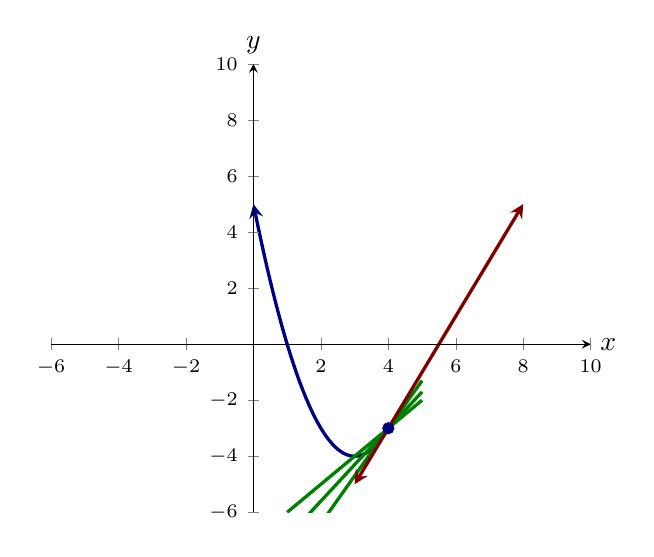
\begin{tikzpicture}
     \begin{axis}[
                domain=-10:10, ymax=10, xmax=10, ymin=-6, xmin=-6,
                axis lines =center, xlabel=$x$, ylabel=$y$,
                ytick={-6,-4,-2,2,4,6,8,10},
                xtick={-6,-4,-2,2,4,6,8,10},
                ticklabel style={font=\scriptsize},
                every axis y label/.style={at=(current axis.above origin),anchor=south},
                every axis x label/.style={at=(current axis.right of origin),anchor=west},
                axis on top,
                ]


        \addplot [draw=penColor, very thick, smooth, domain=(0:4),<-] {(x-3)^2 - 4};

        \addplot [color=penColor,only marks,mark=*] coordinates{(4,-3)};
        
       


        \addplot [draw=penColor4, very thick, smooth, domain=(1:5)] {(x-4)-3};
        \addplot [draw=penColor4, very thick, smooth, domain=(1:5)] {1.3*(x-4)-3};
        \addplot [draw=penColor4, very thick, smooth, domain=(1:5)] {1.7*(x-4)-3};



          \addplot [draw=penColor2, very thick, smooth, domain=(3:8),<->] {2*(x-4)-3};



        %\node[penColor] at (axis cs:5,-4) {$(h, k)$};
        %\node[penColor] at (axis cs:5,-9) {$-0.5 x^2 - 5 x + 15.5$};



    \end{axis}
\end{tikzpicture}
\end{image}


The secant lines on the left smoothly turn into the tangent line as you move to the right. \\


There are no secant lines on the right, so we don't have to worry about them. \\





In this case, we have a one-side tangent line.  \\

We have a one-side derivative. \\


For the function above, we have a \textbf{left derivative}.












Similarly, we might have a one-side tangent line on the right.  \\

We would have a one-side derivative. \\


We would have a \textbf{right derivative}.









\begin{definition} \textbf{\textcolor{green!50!black}{Derivative}}  (two-sided)


Suppose we have a really nice situation.


\begin{itemize}
\item We have a function, $f$, 
\item We have a domain number, $t_0$, 
\item This domain number is inside an open interval inside the domain.  $t_0 \in (a, b) \subset Domain$. 
\item The secant lines on both sides of $(t_0, f(t_0))$ are smoothly approaching the same line from both sides.
\end{itemize}

Then, there is a tangent line to the graph of $f$ and the secant lines on both sides are smoothly turning into this tangent line at the tangent point $(t_0, f(t_0))$. \\

The slope of this tangent line is the value of the \textbf{derivative} of $f$ at $t_0$.

\[
iRoC(t_0) =f'(t_0) = \text{slope of tangent line}
\]


\begin{itemize}
  \item If the tangent line doesn't have a slope, then the derivative has no value there. The derivative does not exist at $t_0$.

  \item If the secant lines on both sides are not smoothly agreeing, then there is no tangent line at $(t_0, f(t_0))$ and the derivative does not exist at $t_0$.   
\end{itemize}

\end{definition}

\textbf{Note}: The term ``derivative" implies a two-sided derivative.  Otherwise, we would say `right' or `left'. \\




\begin{warning}

Saying the word ``derivative'' implies two sides. \\

For the derivative to exist at a domain number, the corresponding point on the graph must have secants approaching on both sides. \\


This means that end-point numbers for domain intervals are automatically critical numbers.  The derivative cannot exist at end-points, even if there is a one-sided tangent line, because ``derivative'' means two sides. \\

\end{warning}




So, we have two separate situations. \\


We have a domain number inside an open interval in the domain, so that there are two sides. Since, it is a domain number, we know there is a point on the graph of the function and the graph is on both sides.  We can examine if there is a tangent line or not and if it has a slope or not. \\

A different situation is a domain number that is the end of an interval in the domain.  The domain number only has one side in the domain.  This automatically disqualifies the function from having a derivative value at this domain number.  The domain number is a critical number.  However, this is still a nice situation, which we would like to describe. \\

We would still like to describe one-sided situations. \\

There can still be a tangent line, a one-sided tangent line. That tangent line can still have a slope. \\

So, we also have a one-sided derivative, which is like half of a derivative. \\











\begin{definition} \textbf{\textcolor{green!50!black}{Left Derivative}}  (one-sided) 


Suppose we have a really nice one-sided situation.


\begin{itemize}
\item We have a function, $f$, 
\item We have and a domain number, $t_0$, 
\item This domain number is inside an interval (half open) inside the domain of the form  $t_0 \in (a, t_0] \subset Domain$. 
\item The secant lines on the left side of $(t_0, f(t_0))$ are smootlhy approaching the same line.
\end{itemize}

Then, there is a tangent line to the graph of $f$ and the secant lines on the left side are smoothly turning into this tangent line at the tangent point $(t_0, f(t_0))$. \\

The slope of this tangent line is the value of the \textbf{left derivative of $f$ at $t_0$}. \\

We have a function called the left derivative of $f$ or the left $iRoC_f$.

\[
iRoC_{f_{-}}(t) =f'_{-}(t) = \text{slope of tangent line}
\]

The left derivative is symbolized with a subscript of ``-'' with the derivative name. \\
 

\end{definition}






\begin{definition} \textbf{\textcolor{green!50!black}{Right Derivative}}  (one-sided) 


Suppose we have a really nice one-sided situation.


\begin{itemize}
\item We have a function, $f$, 
\item We have and a domain number, $t_0$, 
\item This domain number is inside an interval (half open) inside the domain of the form  $t \in [t_0, b) \subset Domain$. 
\item The secant lines on the right side of $(t_0, f(t_0))$ are smoothly approaching the same line.
\end{itemize}

Then, there is a tangent line to the graph of $f$ and the secant lines on the right side are smoothly turning into this tangent line at the tangent point $(t_0, f(t_0))$. \\

The slope of this tangent line is the value of the \textbf{right derivative of $f$ at $t_0$}.


We have a function called the right derivative of $f$ or the right $iRoC_f$. \\

\[
iRoC_{f_{+}}(t) =f'_{+}(t) = \text{slope of tangent line}
\]


The right derivative is symbolized with a subscript of ``+'' with the derivative name. \\ 

\end{definition}



\textbf{Note:} It is possible that we have a domain number where there is both a left and right derivative value and they are different values.  In this case, there would be no value of the derivative.  If there is a derivative value, then the left and right sides must match.  We saw this with an absolute value function.





\subsection*{No Side}


If the domain number is isolated, meaning no domain numbers immediately to the left or right, then there just is no derivative there. \\

The term derivative implies that there is some sort of approaching.




















\begin{center}
\textbf{\textcolor{green!50!black}{ooooo-=-=-=-ooOoo-=-=-=-ooooo}} \\

more examples can be found by following this link\\ \link[More Examples of Quadratic Behavior]{https://ximera.osu.edu/csccmathematics/precalculus1/precalculus1/quadraticBehavior/examples/exampleList}

\end{center}




\end{document}




